\chapter{Dataset\label{ch:Dataset}}
\section{Dimensions and Size }
In this section, we will explore the size and dimension of the dataset. How it is stored in the storage. Moreover, we are going to know, how dataset is built. How many instances are there? What does an instance look like? And much more.
\subsection{ Size: }
The dataset consists of 4 sentences (initially) to reflect the working and performance of the system being developed. The four sentences of Urdu are:
\begin{enumerate}
  \item Khush-Aamdeed.
  \item Ap kese hain ?
  \item Apka naam kia hai ? 
  \item Allah Hafiz 
\end{enumerate}

So dataset contains samples from each sentence. To create a balanced dataset, we’ve taken 22 instances of each class (sentence). Each instance is a video of sign being performed in front of Kinect camera. Each video is stored in form of an Excel file with each record representing a frame of the video. Length of videos is variable i.e. a sign may long 2 seconds and some other may long for 3 seconds. For a class, there may also be variable video lengths. Each file consists a number of rows representing frames in the video.
\subsection{ Basic unit }
Each video contains 'N' number of frames. 'N' varies from video to video and further varies from sign to sign. Each frame record contains 'M' number of features from the corresponding frame. These features of frames are the basic units of which an instance is composed of. 'M' varies from frame to frame. All the features from the frames of the videos are numeric and quantifiable.

\section{ Analysis: }
In this section, we will analyze the significance of dataset for building some model. We will see how well the dataset instances generalize a sign? How missing data occurs? What potential effects it can pose to the machine learning? How missing values are handled? All this analysis will be done in the following section.
\subsection{ Generalization }
For the generalization purpose, we've taken the signs from 3 different signers so that system does not over fits a single person. Each signer has performed 8 signs. Moreover, the video length is also variable that introduces some degree of generalization to dataset.
\subsection{ Missing Values }
As discussed, the feature length for a frame is variable. So for a file, there are frames stacked to each other in the xlsx file. So for a feature 'X' in a feature vector of frame 'A', 'X' may not be present in another frame 'B' causing a missing value (NA). Our dataset in contains a bundle of missing values and dataset is very noisy. Moreover, due to the variance in the length of the feature vector, it becomes very difficult to handle and use this data to make a model due to difficulty in data imputation.
\begin{figure}[!htb]
  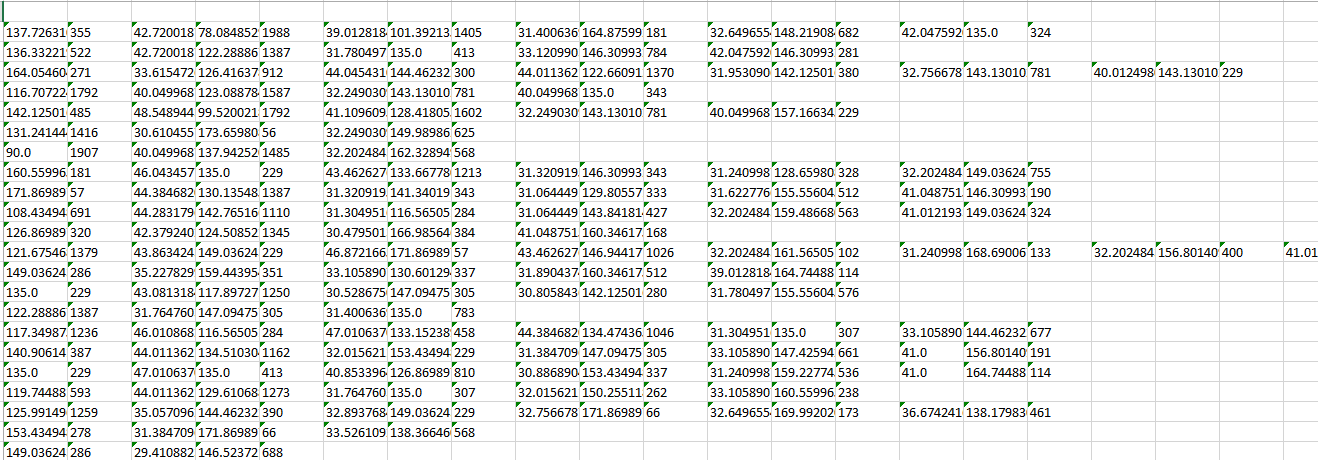
\includegraphics[height=6cm,width=15cm]{ThesisFigs/dataset1}
  \caption{Missing values in Dastsets }\label{fig:dataset1}
\end{figure}
\newline Above figure shows the missing values in as blank records.
\clearpage
\subsection{ Missing Records }
As video length is variable, so a video 'A' may have 'N' number of frames and another video 'B' may have 'P' number of frames. The difference between 'P' and 'N' is the missing frames length in the corresponding video.
\begin{figure}[!htb]
  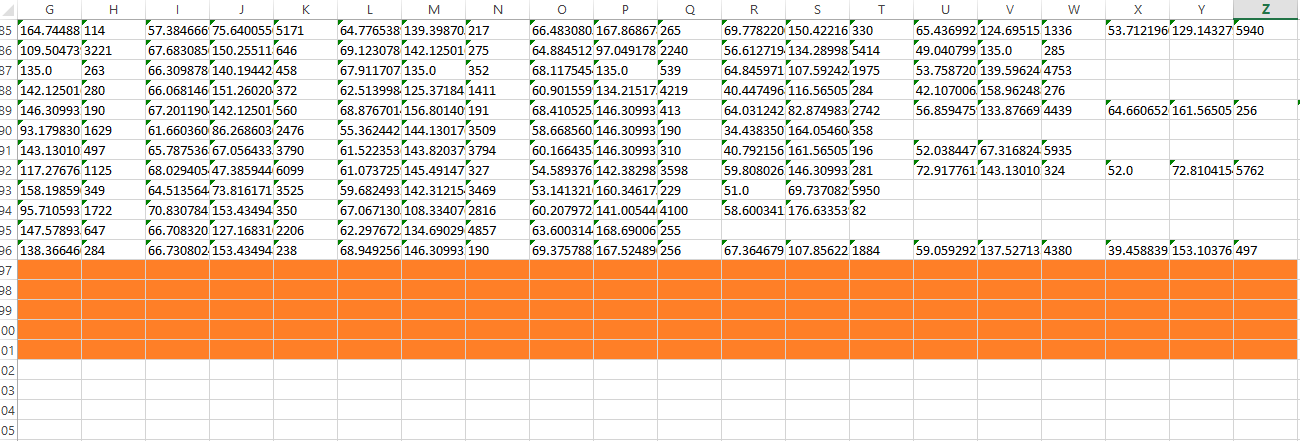
\includegraphics[height=6cm,width=15cm]{ThesisFigs/dataset2}
  \caption{Missing records in Dastsets }\label{fig:dataset2}
\end{figure}
\section{ Padding}
In order to do machine learning on the dataset we need each instance to be in the same shape and size. To achieve this purpose, we pad our data instances with zero.
\subsection{ Feature Padding }
We first find the maximum length feature vector. Then we pad each of the record with length less than the maximum length with zero to make compatible to the maximum length feature.
\subsection{ Frame padding}
And lastly, we pad each video with zero vectors so that to make it equal to the length of maximum length video.
